%================ch1======================================
\chapter{Introduction}\label{ch:ch1}
LaTeX is a high-quality typesetting system; it includes features designed for the production of technical and scientific documentation. LaTeX is the de facto standard for the communication and publication of scientific documents. LaTeX is available as free software.

LaTeX is widely used in academia for the communication and publication of scientific documents in many fields, including mathematics, statistics, computer science, engineering, chemistry, physics, economics, linguistics, quantitative psychology, philosophy, and political science. It also has a prominent role in the preparation and publication of books and articles that contain complex multilingual materials, such as Tamil, Sanskrit and Greek. LaTeX uses the TeX typesetting program for formatting its output, and is itself written in the TeX macro language. See figure~\ref{fig:im1}, \ref{fig:im2} of \ref{fig:subfigs cap}

LaTeX is intended to provide a high-level language that accesses the power of TeX in an easier way for writers. In short, TeX handles the layout side, while LaTeX handles the content side for document processing. LaTeX comprises a collection of TeX macros and a program to process LaTeX documents. Because the plain TeX formatting commands are elementary, it provides authors with ready-made commands for formatting and layout requirements such as chapter headings, footnotes, cross-references and bibliographies.
%%
\begin{figure}
	\centering
	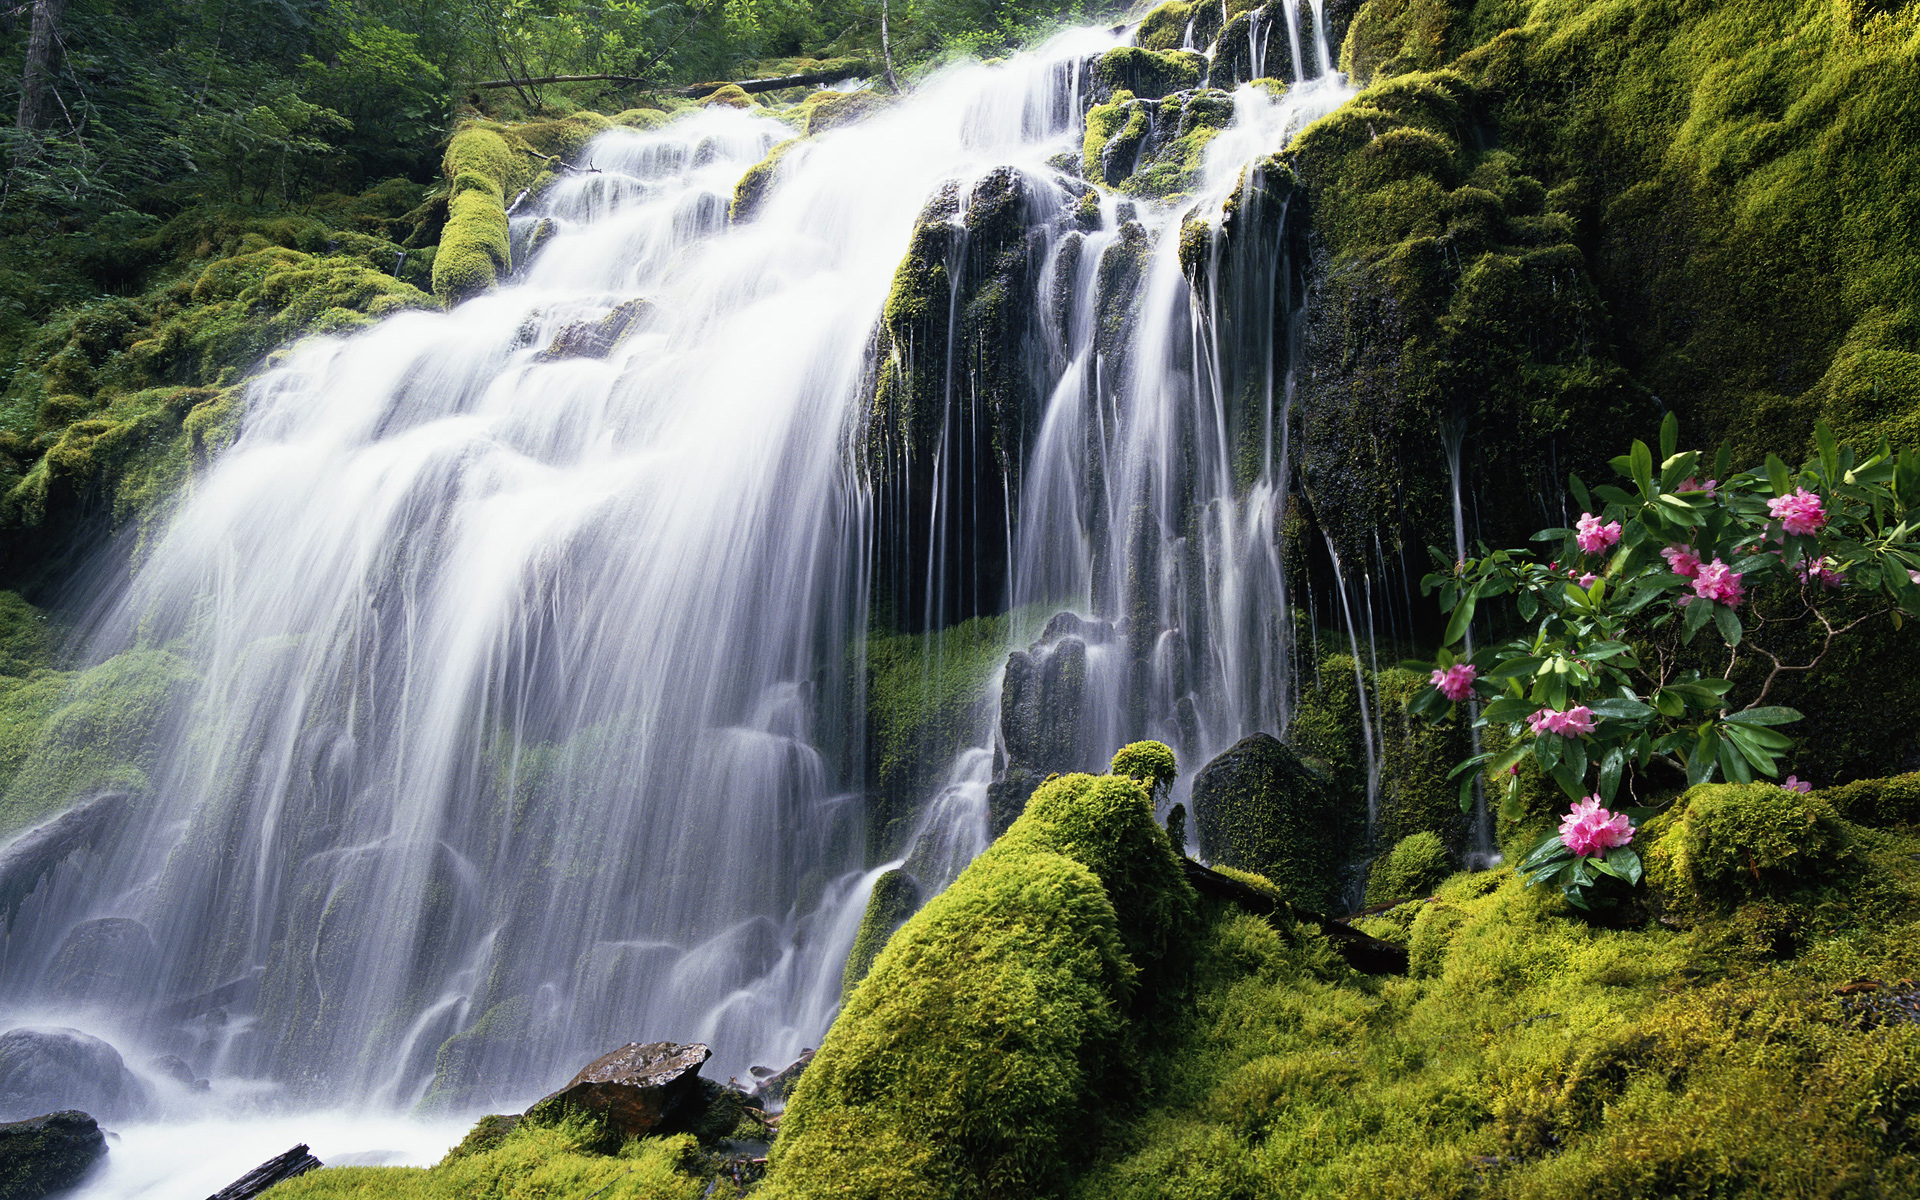
\includegraphics[width=0.7\linewidth]{image2}
	\caption{Caption of fig. 1.}
	\label{fig:image2}
\end{figure}

In order to create a document in LaTeX, you first write a file, say document.tex, using your preferred text editor. Then you give your document.tex file as input to the TeX program (with the LaTeX macros loaded), and TeX writes out a file suitable for viewing onscreen or printing. This write-format-preview cycle is one of the chief ways in which working with LaTeX differs from what-you-see-is-what-you-get word-processing. It is similar to the code-compile-execute cycle familiar to computer programmers. Today, many LaTeX-aware editing programs make this cycle a simple matter of pressing a single key, while showing the output preview on the screen beside the input window. Some online LaTeX editors automatically refresh the preview. Other online tools provide incremental editing in-place, mixed in with the preview in a streamlined single window.

\section{Subfigure}
A useful extension is the subcaption package, which uses subfloats within a single float. The subfig package (subfigure package is deprecated) is a useful alternative when used in-conjunction with LaTeX templates (i.e. templates for journals from Springer and IOP, IEEETran and ACM SIG) that are not compatible with subcaption. These packages give the author the ability to have subfigures within figures, or subtables within table floats. Subfloats have their own caption, and an optional global caption.

\begin{figure}
\centering
\begin{subfigure}[b]{0.45\textwidth}
  \centering
  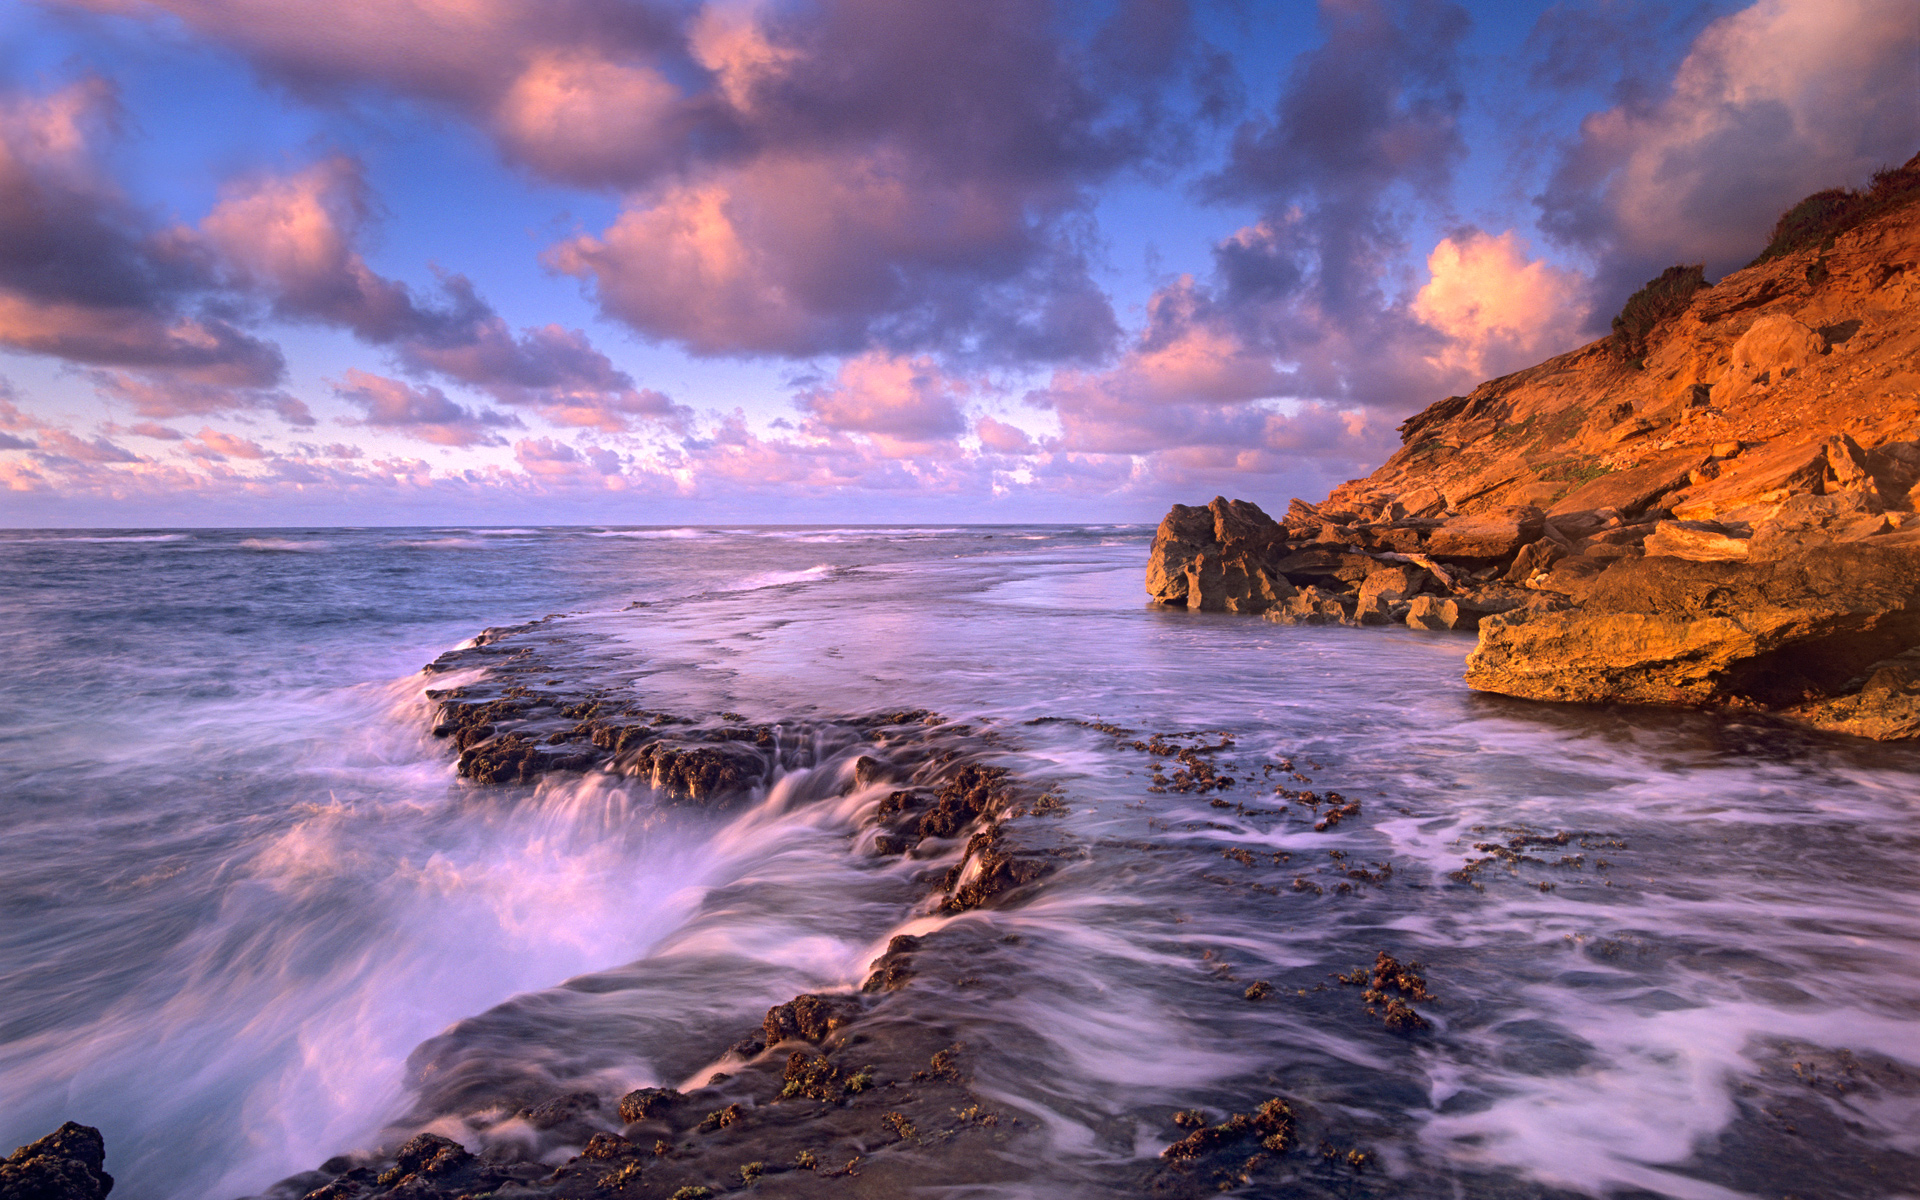
\includegraphics[width=\textwidth]{image1}
  \caption{}
  \label{fig:im1}
 \end{subfigure}
~
\begin{subfigure}[b]{0.45\textwidth}
  \centering
  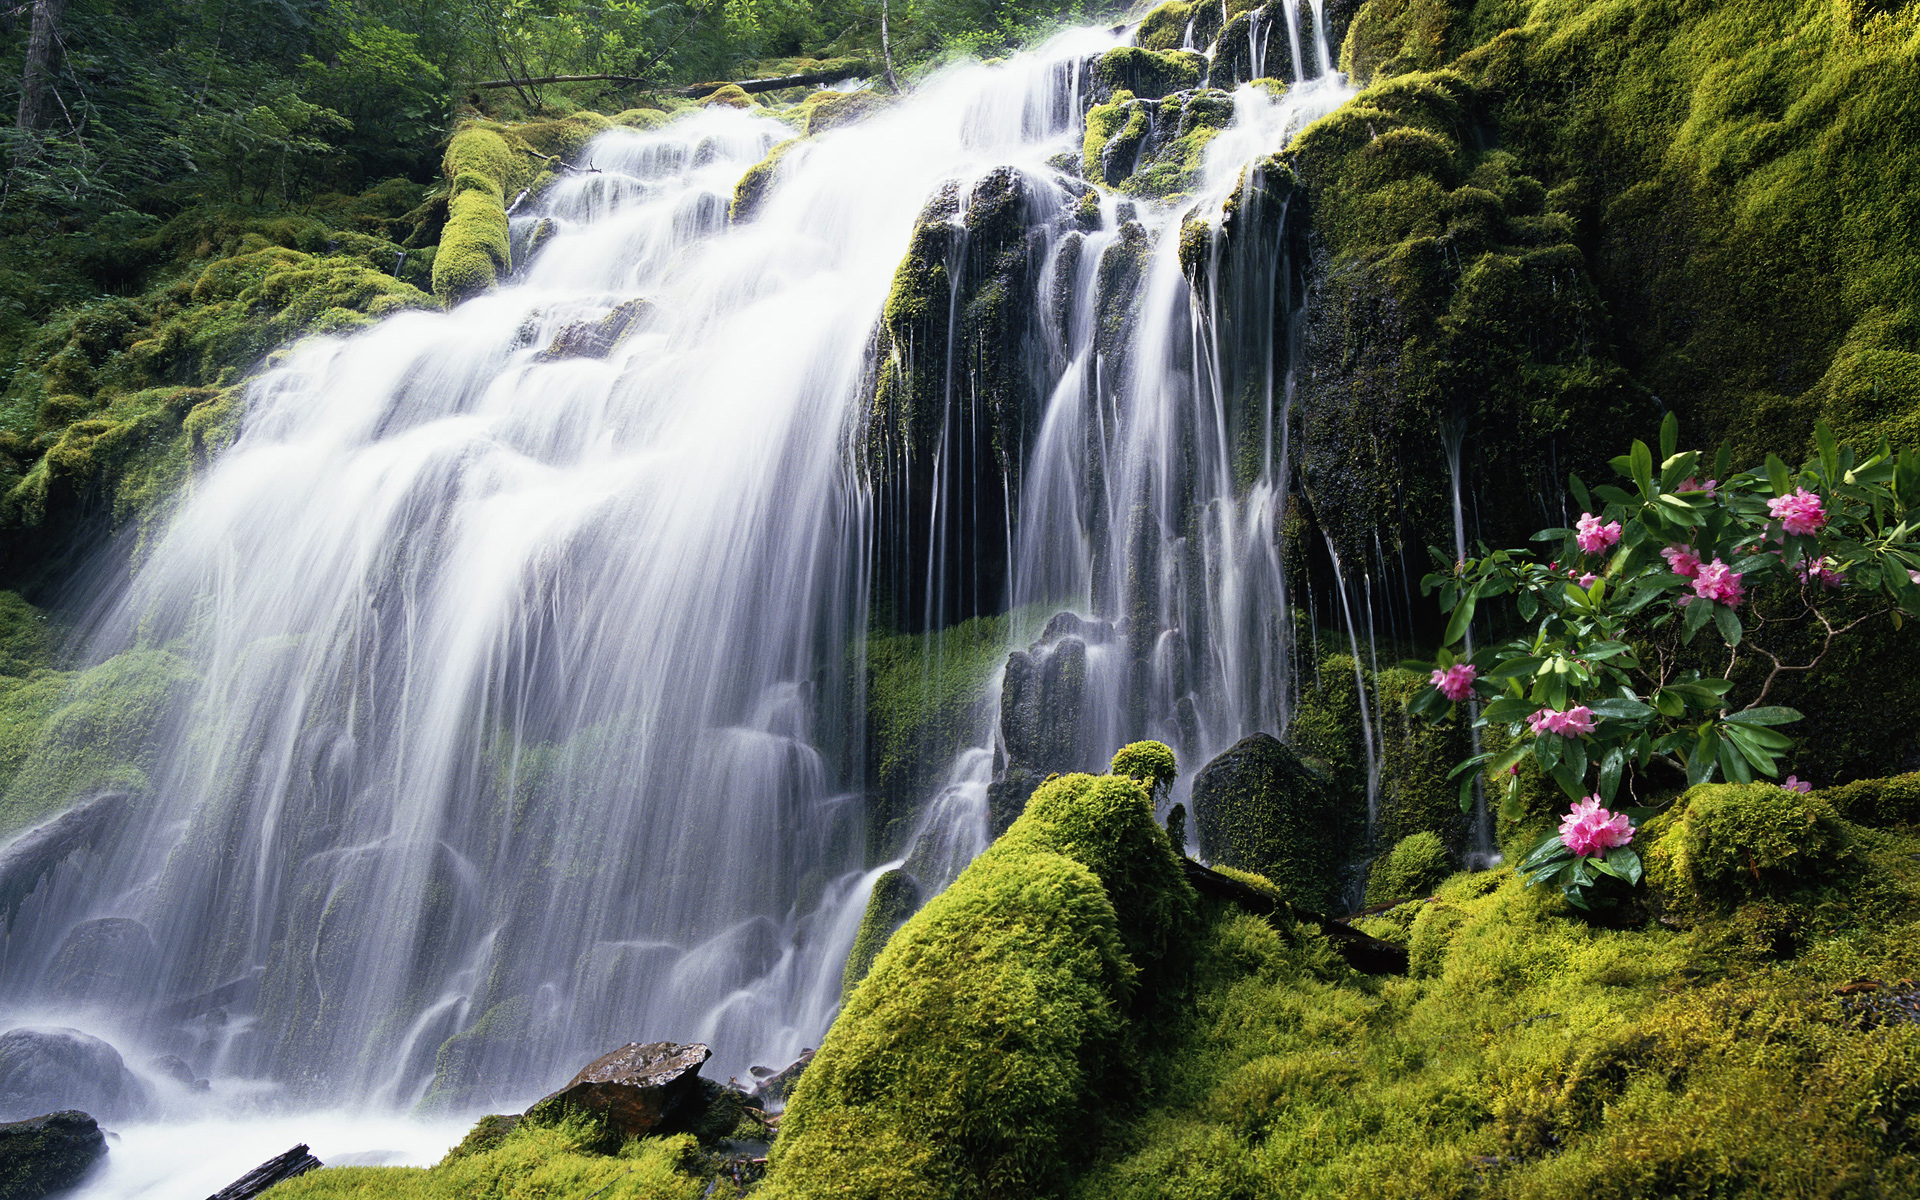
\includegraphics[width=\textwidth]{image2}
  \caption{}
  \label{fig:im2}
\end{subfigure}
\caption{Two figure side by side}
\label{fig:subfigs cap}
\end{figure}

\section{Table}
Tables are a common feature in academic writing, often used to summarize research results. Mastering the art of table construction in LaTeX is therefore necessary to produce quality papers and with sufficient practice one can print beautiful tables of any kind.

Keeping in mind that LaTeX is not a spreadsheet, it makes sense to use a dedicated tool to build tables and then to export these tables into the document. Basic tables are not too taxing, but anything more advanced can take a fair bit of construction; in these cases, more advanced packages can be very useful. However, first it is important to know the basics. Once you are comfortable with basic LaTeX tables, you might have a look at more advanced packages or the export options of your favorite spreadsheet. Thanks to the modular nature of LaTeX, the whole process can be automated in a fairly comfortable way. Table~\ref{tab: sample}.

\begin{table}
\centering
\caption{Random table}
\label{tab: sample}
\begin{tabular}{|c|c|c|c|c|c|c|}
\hline 
1 & 2 & 3 & 4 & 2 & 3 & 4 \\ \hline 
5 & 6 & 7 & 8 & 2 & 3 & 4 \\ \hline 
9 & 10 & 11 & 12 & 2 & 3 & 4\\ \hline 
13 & 14 & 15 & 16 & 2 & 3 & 4\\ \hline 
\end{tabular} 
\end{table}









